\documentclass[11pt]{extarticle}
\usepackage{apacite, setspace}
\usepackage[margin=1in]{geometry}
%\usepackage{times}
\usepackage{setspace}
\usepackage{float}
\usepackage{subfig}
\usepackage{tikz}
\usepackage{titlesec}
\usepackage{booktabs} % To thicken table lines
\usepackage[shortlabels]{enumitem}
\usepackage{amsthm,amssymb} % for proof 
\usepackage[bottom]{footmisc} %for footnote to bottom
\usepackage{amsmath}
\usepackage{cancel}

\usepackage{mathtools} % for auto \left( \right)

\DeclarePairedDelimiter\autobracket{(}{)}
\newcommand{\br}[1]{\autobracket*{#1}}


\usepackage{amsfonts}
% image
\usepackage{graphicx}
\graphicspath{ {img/} }

\usepackage{array}
\newcolumntype{L}[1]{>{\raggedright\let\newline\\\arraybackslash\hspace{0pt}}m{#1}}
\newcolumntype{C}[1]{>{\centering\let\newline\\\arraybackslash\hspace{0pt}}m{#1}}
\newcolumntype{R}[1]{>{\raggedleft\let\newline\\\arraybackslash\hspace{0pt}}m{#1}}


\titlespacing*{\section}
{0pt}{0px}{0px}


% image
\usepackage{graphicx}
\graphicspath{ {img/} }

% for header
\usepackage{fancyhdr}
\pagestyle{fancy}
\lhead{\textbf{ELEC 321 -- Stochastic Signals \& Systems: Homework 2}}
\rhead{Charles Clayton \texttt{\#21518139} }
\cfoot{\thepage} 
\renewcommand{\headrulewidth}{0.4pt}
\renewcommand{\footrulewidth}{0.4pt}
 

 
% for indenting verbating
\usepackage{fancyvrb}

\setlength{\parskip}{\baselineskip}

% automatically convert "" to ``''
\usepackage [autostyle, english = american]{csquotes}
\MakeOuterQuote{"}

\begin{document}

%\pagenumbering{gobble}
\singlespacing

%$$\br{\frac{1}{2}} + \br{1} - \br{\frac{\int_0^{2\pi} f(x)}{\sqrt[2]{\frac{1}{2}}}}$$



\subsubsection*{Problem 1}

The probability of a test being positive $p'$ is given by sensitivity = $P(T | F) = 0.90$, and specificity = $P(T^c | F^c) = 0.98$, where $P(F^c) = 1- p$, $P(F) = p$.\begin{align*}
p' & = P(test\ positive) \\
& = P(F)P(T|F) + P(F^c)P(T|F^c) \\
& = 0.01(0.90) + (1-0.01)(1 - 0.98)  \\
& = 0.0288
\end{align*}

So for this question, instead of using $p$, the probability an item is defective. We will be using $p'$, the probability the test is positive. Originally I used $p$, and in case I am now misunderstanding the problem, here are my results for that:

\begin{table}[H]
\scriptsize
\centering
\begin{tabular}{rrr}
\toprule
$\mathbf{m}$  & $\mathbf{E(X)}$ & $\mathbf{Var(X)}$ \\
\midrule
1000	&	5004.784	&	1079.235	\\
500	&	2488.574	&	40795.699	\\
200	&	871.020	&	116029.122	\\
100	&	321.984	&	58013.167	\\
50	&	103.748	&	14935.858	\\
25	&	32.772	&	2700.239	\\
20	&	23.209	&	1489.352	\\
10	&	9.781	&	216.188	\\
8	&	8.090	&	114.059	\\
5	&	6.225	&	29.130	\\
\bottomrule
\end{tabular}
\quad 
\begin{tabular}{rrrrr}
\toprule
$\mathbf{j}$ & $\mathbf{k}$ & $\mathbf{m}$  & $\mathbf{E(T_k)}$  & $\mathbf{Var(T_k)}$ \\
\midrule
1	&	10	&	1000	&	50047.841	&	10792.346	\\
2	&	20	&	500	&	49771.476	&	815913.974	\\
3	&	50	&	200	&	43551.016	&	5801456.079	\\
4	&	100	&	100	&	32198.383	&	5801316.660	\\
5	&	200	&	50	&	20749.697	&	2987171.573	\\
6	&	400	&	25	&	13108.932	&	1080095.577	\\
7	&	500	&	20	&	11604.653	&	744675.895	\\
\textbf{8}	&	\textbf{1000}	&	\textbf{10}	&	$\boxed{\mathbf{9780.896}}$	&	\textbf{216187.844}	\\
9	&	1250	&	8	&	10112.765	&	142573.847	\\
10	&	2000	&	5	&	12450.498	&	58259.969	\\
\bottomrule
\end{tabular}
\end{table}

Now continuing assuming we should be using $p'$.

\begin{enumerate}[(a)]
\item 

The probability that $m$ additional tests will be taken is the probability that there is a faulty item in the pool. The probability that no items in $m$ are faulty is $(1-p')^m$, so the probability that at least one item in the pool is faulty is $1-(1-p')^m$. Multiply this by $m+1$ to indicate the initial pool test and the subsequent $m$ item tests. 

If no items in the pool are faulty, $(1-p')^m$, then only one test will be taken so where $X_m = $ cost of testing one pool of size $m$:

$$X_m = \begin{cases} 
5 & \text{with}\ P=(1-p')^m \\
5(m+1) & \text{with}\  P=1 - (1-p')^m  \\
\end{cases}$$

%X_i		5			5(m+1)
%P_i		(1-p)^m		1-(1-p)^m

$$E(X) = \sum_{i=1}^2 X_i P_i$$
$$E(X^2) = \sum_{i=1}^2 X_i^2 P_i$$
$$Var(X) = E(X^2) - E(X)^2$$



\begin{table}[H]
\caption{Mean and Standard Deviation of $X_m$}
\centering
\begin{tabular}{rrr}
\toprule
$\mathbf{m}$  & $\mathbf{E(X)}$ & $\mathbf{Var(X)}$ \\
\midrule
1000	&	5005	&	0	\\
500	&	2504.999	&	2.820	\\
200	&	1002.104	&	2887.190	\\
100	&	478.095	&	12728.742	\\
50	&	197.007	&	11135.028	\\
25	&	69.796	&	3900.979	\\
20	&	49.259	&	2467.043	\\
10	&	17.670	&	472.974	\\
8	&	13.339	&	264.013	\\
5	&	8.399	&	73.413	\\
\bottomrule
\end{tabular}
\end{table}

\item

For $k$ pools, $T_k = X_{m_1} + X_{m_2} + \dots + X_{m_k}$:

$$E(T_k) = \sum_{i=1}^k E(X_{m_i}) = k E(X_m)$$
$$Var(T_k) = \sum_{i=1}^k Var(X_{m_i}) = k Var(X_m)$$





\begin{table}[H]
\caption{Mean and Standard Deviation of $T_j$}
\centering
\begin{tabular}{rrrrr}
\toprule
$\mathbf{j}$ & $\mathbf{k}$ & $\mathbf{m}$  & $\mathbf{E(T_k)}$  & $\mathbf{Var(T_k)}$ \\
\midrule
1	&	10	&	1000	&	50050	&	0	\\
2	&	20	&	500	&	50099.977	&	56.396	\\
3	&	50	&	200	&	50105.221	&	144359.508	\\
4	&	100	&	100	&	47809.473	&	1272874.208	\\
5	&	200	&	50	&	39401.450	&	2227005.660	\\
6	&	400	&	25	&	27918.316	&	1560391.738	\\
7	&	500	&	20	&	24629.582	&	1233521.403	\\
8	&	1000	&	10	&	17670.107	&	472973.746	\\
\textbf{9}	&	\textbf{1250}	&	\textbf{8}	&	$\boxed{\mathbf{16673.317}}$	&	\textbf{330016.246}	\\
10	&	2000	&	5	&	16797.053	&	146826.359	\\
\bottomrule
\end{tabular}
\end{table}



\item The best strategy is where $m = 9$ and $k=1250$.

Using the Python (code in Appendix A), I ran 1000 simulations for each pool size to confirm these results, comparing both the simulated and the calculated costs and graphing the two curves. In Figure 1, the \textit{blue} curve\footnote{If this has been printed in black and white, the observation is that the two curves are almost identical.} represents the costs as calculated using the above formula, and the \textit{red} curve represents the cost as determined by averaging the results the simulations.

\begin{figure}[ht!]
\centering
\begin{tabular}{cc}
  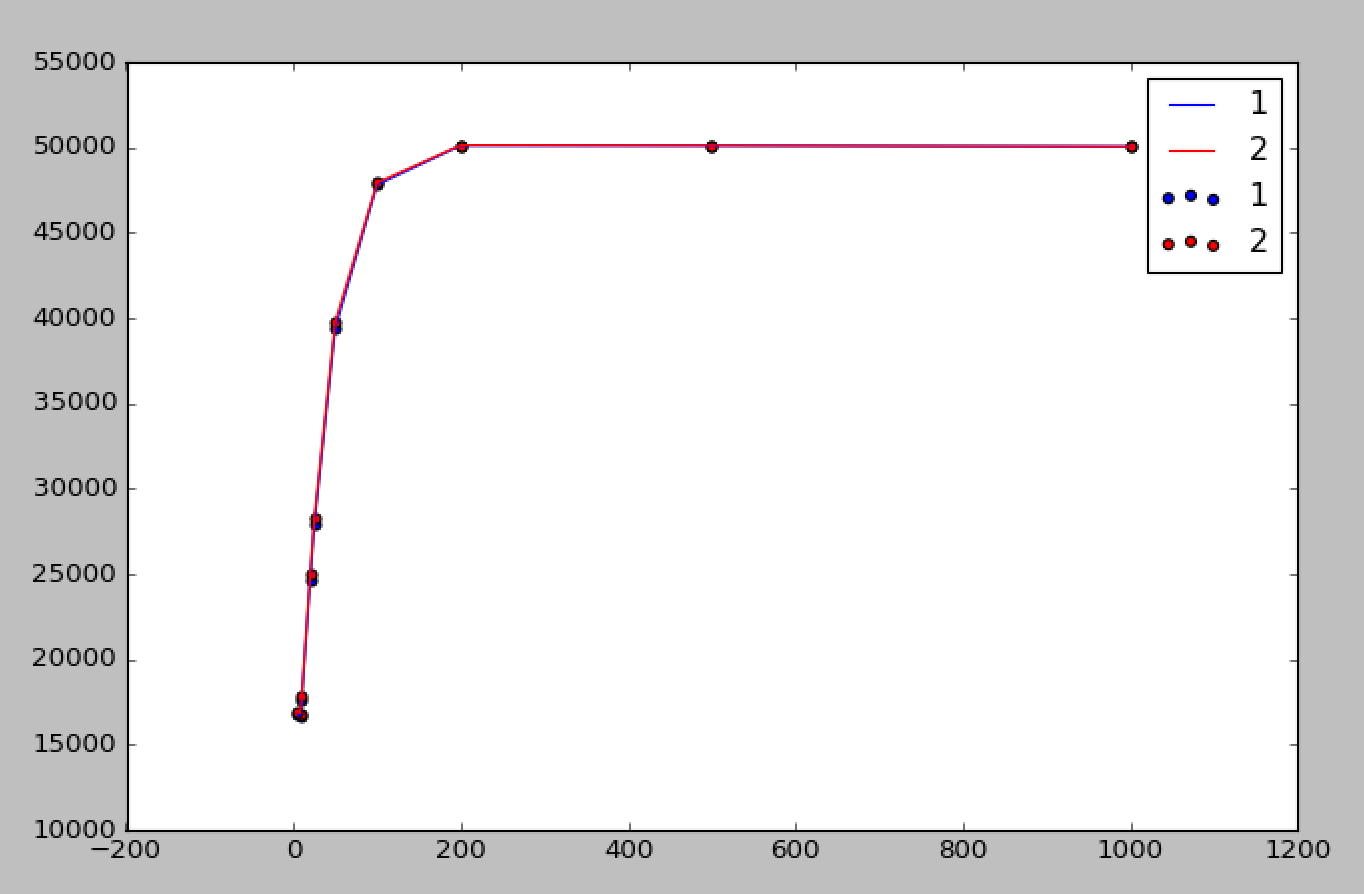
\includegraphics[height=50mm]{P1.png} &   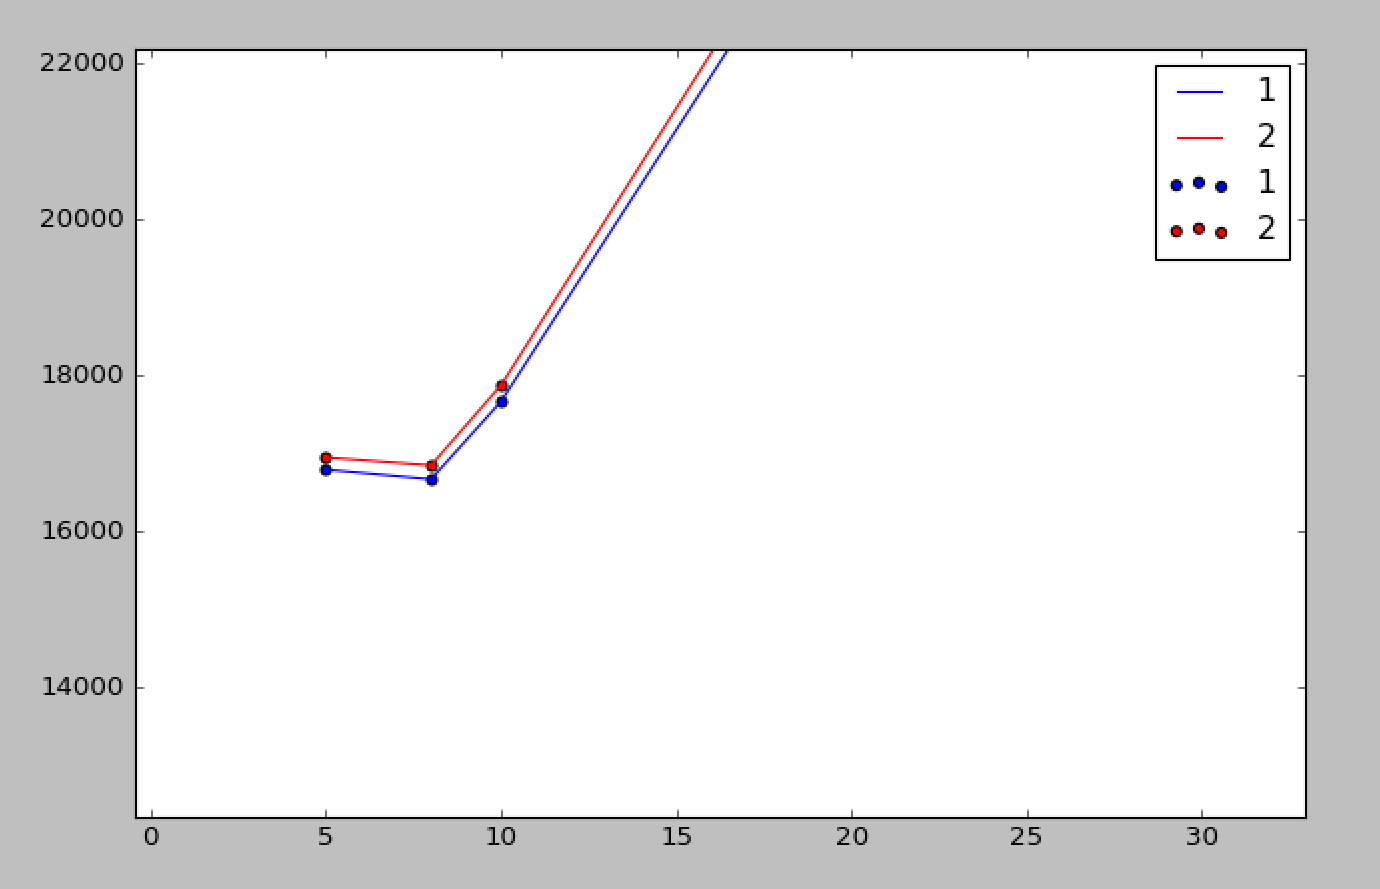
\includegraphics[height=50mm]{P1_2.png} \\
(a) domain $m=[0,1000]$, range $E(T_k)$ & (b) domain $m=[5,30]$, range $E(T_k)$\\[6pt]

\end{tabular}
\caption{Pooling size, $m$ (x-axis) vs. Total cost, $T$ (y-axis)}
\end{figure}


\end{enumerate}



\subsubsection*{Problem 2}

%Probability of success: $p$, and probability of failure: $(1-p)^3$.

%$P($ 3rd failure before 1st success $) = P(F \cap F \cap F) = [P(F)]^3 = (1-p)^3$ 
%Now consider: $P($ 3rd failure before 2nd success $)$ $$SFFFS = {4 \choose 1} p (1-p)^3 $$
%$$FFFFS = (1-p)^4$$ So: $$P(  \text{3rd failure before 2nd success} = (1-p)^4 + {4 \choose 1} p (1-p)^3  $$ 


\begin{enumerate}[(a)]
\item \begin{proof}

In words, consider $P(T_j < S_i)$ as $P($ $j$th failure is before $i$th success $)$ for $i+j-1$ trials. Observe that there will be at least $j$ failures and at most $i-1$ successes, therefore:
$$T_j \geq j$$ $$S_i \leq i-1$$
So where we let $X$ = \# of successes in $i+j-1$ trials, then $$X \sim Bin(i+j-1, p)$$
Therefore:  \begin{align*} 
P(T_j < S_i) = & P(X \leq i-1) \\
= & P(Bin(i+j-1, p) \leq i-1) \\
= & P( Bin(i+j-1, p) \geq i)  \end{align*} \end{proof} To further show the equality stands and validate this logic, I will show that these are equal through simulation. I wrote the Python code in Appendix B to simulate this scenario 5,000,000 times for each  $(i,\ j $).

In each simulation, I created random sequences of trials and determined the value of $S_i$ and $T_j$ to track how often $T_j > T_i$ was true. I also generated a random binomial  and kept track how often $Bin(i+j-1, p) \geq i$. At the end I compared the values to compare the probabilities and they were very, very close.



%$$P(T_j < S_i) = P(Bin(i+j-1, p) \geq i)$$ Where $Bin(i+j-1, p)$ represents a binomial random variable with $i+j-1$ trials and a probability $p$ of success, and $S_i$ represents the $i$th success and $T_j$ the time of the $j$th failure.



 \begin{table}[H]
\caption{Results of Simulation}
\centering
\begin{tabular}{clll}
\toprule
$\mathbf{(i,j)}$ & $\mathbf{P(T_j > S_i)}$ & $\mathbf{P(Bin(i+j-1,p) \geq i)}$ & \textbf{\% Diff}  \\
\midrule
1,2	&	0.1900518	&	0.1900272	&	0.0129438	\\
2,1	&	0.0099282	&	0.0099770	&	0.4915292	\\
5,7	&	0.0027762	&	0.0027478	&	1.0229811	\\
7,5	&	0.0000224	&	0.0000224	&	0	\\
\bottomrule
\end{tabular}
\end{table}

\item 
The CDF of a binomial function is: $$ P(X \leq x) = \sum_{j=0}^{x} {n \choose x} p^x (1-p)^{n-x}$$
Where $n$ = $i+j-1$ and $x=i$. $$ P(Bin(i+j-1,p) < i)) = \sum_{j=0}^{i} {i+j-1 \choose i} p^x (1-p)^{(i+j-1)-i}$$

Given $p=0.10$: \begin{table}[H]
\centering
\begin{tabular}{cl}
\toprule
$\mathbf{(i,j)}$ & $\mathbf{P(T_j < S_i)}$  \\
\midrule
(1,2) & 0.82 \\
(2,1) & 0.98  \\
(5,7) & 0.9877 \\
(7,5) & 0.9998 \\
\bottomrule
\end{tabular}
\end{table}


\item Again using the Python code in Appendix B to run a simulation, I determined the mean and standard deviation of the number of failures to be: $$\mu \approx \boxed{179.98} $$ $$ \sigma \approx \boxed{42.419}$$
%;

%Argue it logically, don't try to use math.

%\begin{align*}
%P(j-th failure < i-th success) = & P(Bin(i+j-1, p) >= i) \\
%P(1st failure < 1st success = & 1-p \\
%\end{align*}

%Represent $Bin(i+j-1, p) >= i) = X$ = \# of successes in i+j-1 trials 

%More than $j$ failures, $Bin(i+j-1, 1-p) > j)$.

%$ X \sim Bin(n, p)$

%X = \# of successes in n independent trials


\end{enumerate}



\subsubsection*{Problem 3}


Let $Y$ represent the number of traffic accidents in a given time $[Y \approx P(\lambda)]$ where $\lambda = 5/\text{day} = 35/week = \frac{5}{24}/hour $

\begin{enumerate}[(a)]
\item  For a Poisson distribution: $$\mu = \sigma^2 = \lambda = 35/week $$


\item $$P(X > 40) = 1 - \sum_{i=0}^{40} P(X = i) = 1 - \sum_{i=0}^{40} \frac{e^{-35}(35^i)}{i!} = \boxed{0.17506}$$

%\item $$P(X > 40) = 1 - \int_{i=0}^{40} P(X = i) = 1 - \int_{i=0}^{40} \frac{e^{-35}(35^i)}{i!} = \boxed{0.19689}$$


\item The probability of waiting less than four hours is the same as the probability that an accident happens in the 0$th$, 1$st$, 2$nd$, or 3$rd$ hour.


% $$ P(X < 4) = P(X=0) + P(X=1) + P(X=2) +  P(X=3)  $$
% $$ = \sum_{i=0}^3 \frac{e^{-\frac{5}{24}} \left( \frac{5}{24} \right)^i}{i!} = 0.99993 $$


% Since there are $5/24 = 0.2083$ accidents per hour, then there is one accident every $24/5 = 4.8$ hours, so this seems incorrect.

% It was unclear to me whether I should start counting from the 0$th$ hour or the $1st$ hour, so as before I simulated the situation in Python to compare my answers.

% $$ P(X < 4) = \int_{t=0}^4 \frac{e^{-\frac{5}{24}}\left( \frac{5}{24} \right)^i}{i!} dt = 0.52048$$


 $$ P(X < 4) = \int_{0}^4 \frac{5}{24} e^{-\frac{5}{24}t} dt = 1-e^{-\frac{5}{6}} = \boxed{0.5654}$$
 



\item $$ \frac{n}{\lambda} = \frac{4}{5/24} = \boxed{19.2 \text{\ hours}} $$

\end{enumerate}

\subsubsection*{Problem 4}


\begin{enumerate}[(a)]

\item When you have independent measurements, then the sample mean estimates $E(X)$ and is: $$\frac{1}{n} \sum_{i=1}^{n} x_i = \overline{x}$$
Therefore $E(X^2)$ is estimated by: $$\frac{1}{n} \sum_{i=1}^{n} x_i^2 = \overline{x^2}$$
And since X is normally distributed:$$X \sim N(\mu, \sigma^2)$$ $$E(X) = \mu$$ $$Var(X) = \sigma^2$$
Then since $Var(X) = E(X^2) - E(X)^2$:
 $$E(X^2) = \sigma^2 + \mu^2$$


So $\boxed{ \hat{\mu} = \overline{x} = 11.96 }$

By the central limit theorem (CLT), if $n \geq 20$, $X_1 \dots X_n$. 

$$\overline{X} \sim N(\mu, \sigma^2/n)$$

Because all measurements have the same expected value:$$\mu = E(X_i)$$ $$\sigma^2 = Var(X_i)$$

And because the more measurements you get $(n)$, the less is the standard area as it converges to the actual $\mu$: 

Then $$n = \sqrt{15} $$

And so: $$SE = \sqrt{ \frac{\sigma^2}{n}} = \frac{\sigma}{\sqrt{n}} = \frac{\sigma}{\sqrt{15}}$$


\item \begin{enumerate}[b1)]

\item 
$$E(X) = \int xf_X(x) dx $$ % = \frac{\alpha}{\lambda}
$$M(X) = E(e^{tx}) = \int_0^{\infty} e^{tx} f_X(x) dx$$

Solve this for $E(X)$ for use in next part.
\item  Since $X$ is a Gamma random variable with density: $$f_X(x) = \frac{\lambda^\alpha}{\Gamma(\alpha)} x^{\alpha -1 } e^{-\lambda x}, \ \ x > 0 $$
Its expected value is: $$E(X) = \frac{\alpha}{\lambda}$$ And the variance is: $$Var(X) = \frac{\alpha}{\lambda^2}$$ Therefore (1): $$\overline{X} = \frac{\hat{\alpha}}{\hat{\lambda}}$$ And (2): $$ \sigma^2 = \frac{\hat{\alpha}}{\hat{\lambda^2}} $$ Solve (1) and (2) for $\hat{a}$ and $\hat{\lambda}$.



\end{enumerate}





%(b3)

%Generate 15 values from gamma distribution with parameters $\Gamma gamma(15, ond then other stuf)$

%Then calculate X bar, then calculate standard deviation. 

%mean(x) = x bar

%sd(x) = sd 

%Repeat 10k

%$\lambda(i) = ...$

%$\alpha(i) = ...$

%Then you'll get a vector of 10k estimates for alpha and lambda, then average two things using.

%Plot histograms of them to see how they look.

\end{enumerate}


\subsubsection*{Problem 5}


Where $U$ is a uniform random variable on the interval (0, 1) and $ X = -\ln(1-U)/\lambda $

\begin{enumerate}[(a)]
\item \begin{proof}

%Notice the domain of X is $(-\infty,1)$ so $F_X(x) = 0$ for $x \geq 1$.

%For $x < 1$: $$ F_X(x) = P(X \leq x) = P \left( - \frac{\ln(1-U)}{\lambda} \leq x \right) = P( U \geq 1-e^{-\lambda x} ) = 1 - F_U(1-e^{-\lambda x} ) $$

%Since $U$ is uniform, then $F_U(x) =x $, so: $$ F_X(x) = 1 - (1-e^{-\lambda x} ) = e^{-\lambda x}$$

%For a uniform distribution:
%$$f(X) = \begin{cases}
%		0 & x \leq \alpha \\
%		1/(\beta - \alpha) & \alpha < x < \beta \\
%		0 & x \geq \beta \\
%	\end{cases}$$

%$$F_X(x) = \begin{cases}
%		0 & x \leq \alpha \\
%		\frac{1}{\beta - \alpha} \int_{\alpha}^{x} dt = \frac{x-\alpha}{\beta-\alpha} & \alpha < x < \beta \\
%		1 & x \geq \beta \\
%	\end{cases}$$
	
%$$ \mu = \frac{\alpha + \beta}{2},\  \ \ \mu_2 = \frac{\beta^2 + \alpha^2 + \alpha \beta}{3}   $$	

%$$ \sigma^2 = \mu_2 - \mu^2 = \frac{(\beta - \alpha)^2}{12}	$$
	
%Where $\alpha = 0$ and $\beta=1$:

%$$F_X(x) = \frac{x-1}{1-0}$$


Notice that the range of $X$ is $(-\infty, 1)$, so for $x > 1$: $$ F_X(x) = 0$$

For $x \leq 1$: \begin{equation} 
\begin{split} F_X(x) & =  P(X \leq x) \\ 
& = P( -\ln(1-U)/\lambda \leq x)  \\
& = P(U \leq 1-e^{-\lambda x}) \\
& = F_U(1-e^{-\lambda x}) 
\end{split}
\end{equation}
 Since $U$ is Unif$(0, 1)$, then $ F_U(u) = u,\ 0 \leq u \leq 1 $, so: $$ \boxed{F_X(x)  = 1- e^{-\lambda x}} $$ 

$$ f_X(x) = \frac{\partial}{\partial x} F_X(x) = \lambda e^{- \lambda x} $$

% Blah: $$ E(X) = \frac{1}{\lambda} $$ $$ Var(X) = \frac{1}{\lambda^2} $$

Mean: $$ \mu = E(X) = \int_{0}^{\infty} x f_X(x) dx = \int_{0}^{\infty} x \lambda e^{- \lambda x} dx  $$ 
$$ =  -x e^{-\lambda x}\Big|_0^\infty + \frac{-1}{\lambda} e^{-\lambda x} \Big|^\infty_0 = \boxed{\frac{1}{\lambda} } $$

Variance: $$ \sigma^2 = Var(X) = E(X^2) - E(X)^2  $$ $$=  \left( \int_{0}^{\infty} x^2 \lambda e^{- \lambda x} dx  \right) - \left( \frac{1}{\lambda} \right)^2 $$ 

$$ = \left( \frac{2}{\lambda^2} \right)  - \left( \frac{1}{\lambda} \right)^2 = \boxed{\frac{1}{\lambda^2}} $$


\end{proof}

\item 

%$$Y = \left( X-\frac{1}{2} \right)^2 = \left( -\frac{\ln(1-U)}{\lambda} - \frac{1}{2} \right)^2 = \frac{(\lambda + 2 \ln(1-U))^2}{4\lambda^2}$$

%The range of $Y$ is $(-\infty, 1)$, so for $y>1$: $$F_Y(y) = 0$$
%For $y \leq 1$: $$F_Y(y) = P(Y \leq y) = P \left(\frac{(\lambda + 2 \ln(1-U))^2}{4\lambda^2} \leq y  \right) = P \left(\frac{(\lambda + 2 \ln(1-U))^2}{4\lambda^2} \leq y  \right)$$


%Steps for random variable transform:

Let: $$Y=\left(X-\frac{1}{2} \right)^2$$

As before: $$F_X(x) = 1-e^{-\lambda x} > 0,\ \ \text{for}\ x \geq  0$$

% -- exponential density decay

%Plot it.

%Any function of random variable is random variable. Range is value it can take with probability.


Therefore: $$ f_X(x) =
	\begin{cases}
		 \lambda e^{-\lambda x}, & \text{if}\  x \geq 0 \\
		0, & \text{otherwise}
	\end{cases}
$$

For $y < 0$, $F_Y(y) = 0$. So the range is $\boxed{ [0, \infty) }$

\begin{align*}F_Y(y) = P(Y \leq y) & = P\left( \left(X-\frac{1}{2} \right)^2\leq y\right) \\
& = P \left( -\sqrt{y}+\frac{1}{2} \leq x \leq \frac{1}{2} + \sqrt{y} \right) \\
& = P \left( X \leq \sqrt{y} + \frac{1}{2} \right) - P \left(X \leq \frac{1}{2} - \sqrt{y} \right) \\
& = F_X \left(\sqrt{y}+\frac{1}{2} \right) - F_X \left(-\sqrt{y} + \frac{1}{2} \right)
\end{align*}


%So points on 1/2 - sqrt(y) and 1/2 + sqrt(y) are the two x points, and on decaying function we're looking for probability between these x axis points.

%$F_X(\sqrt{y}+1/2) - F_X(-\sqrt{y} + 1/2)$

These are equivalent up until a certain point, then not anymore because function is cut-off at Y axis. The y-intercept is at $y=\frac{1}{4}$, so the above is only valid for $0 \leq y \leq \frac{1}{4}$.
$$\boxed{F_Y(y)  = \begin{cases} 
F_X \left(\sqrt{y}+\frac{1}{2} \right) - F_X \left(-\sqrt{y} + \frac{1}{2} \right) & 0 \leq y \leq \frac{1}{4} \\
F_X \left(\sqrt{y}+\frac{1}{2} \right) & y > \frac{1}{4} \\
\end{cases}}$$
Into order to differentiate this, we will leave it in the form: $$F_Y(y)  = \begin{cases} 
\left( 1-e^{-\lambda \left( \sqrt{y} + \frac{1}{2} \right)} \right) - \left( 1-e^{-\lambda \left( -\sqrt{y} + \frac{1}{2} \right)} \right) & 0 \leq y \leq \frac{1}{4} \\
1-e^{-\lambda \left( \sqrt{y} + \frac{1}{2} \right)} & y > \frac{1}{4} \\
\end{cases}$$
So the PDF is:$$\boxed{ f_Y(y) = \frac{\partial}{\partial y} F_Y(y) = \begin{cases} 
\left( \frac{1}{2 \sqrt{y}} \lambda e^{-\lambda \left( \sqrt{y} + \frac{1}{2} \right)} \right) - \left( \frac{1}{2 \sqrt{y}} \lambda e^{-\lambda \left( \sqrt{y} - \frac{1}{2} \right)} \right) & 0 \leq y \leq \frac{1}{4} \\ \frac{1}{2 \sqrt{y}} \lambda e^{-\lambda \left( \sqrt{y} + \frac{1}{2} \right)}  & y > \frac{1}{4} \\
\end{cases} }$$
To determine the mean, integrate this. This becomes too computationally extensive so I will leave it in the general form, and explain the process. $$\mu =  E(Y) = \int yf_Y(y) dy$$ 
Integrate the PDF piecewise, calling each integral $I$: \begin{align*}
I_1(\lambda) & = \int_\frac{1}{4}^{\infty} \frac{y}{2 \sqrt{y}} \lambda e^{-\lambda \left( \sqrt{y} + \frac{1}{2} \right)} dy  \\ 
I_2(\lambda) & = \int_0^{\frac{1}{4}} \left( \frac{1}{2 \sqrt{y}} \lambda e^{-\lambda \left( \sqrt{y} + \frac{1}{2} \right)} \right) - \left( \frac{1}{2 \sqrt{y}} \lambda e^{-\lambda \left( \sqrt{y} - \frac{1}{2} \right)} \right) dy   \end{align*}
And add the results to determine the mean: $$\boxed{E(Y)  = I_1(\lambda) + I_2(\lambda)}$$
Variance: $$ \boxed{Var(Y) = E(Y^2) - E(Y)^2  = \left( \int y^2f_Y(y) dy  \right) - \br{ I_1(\lambda) + I_2(\lambda) }^2 }$$ 


\end{enumerate}



\subsubsection*{Problem 6}


Suppose the lifetime $Y$ of a system has failure rate $h(y) = (y-5)^2$, $0<y<10$.

\begin{enumerate}[(a)]
\item The failure rate decreases for $0<y<5$, then increases for $5<y<10$.  Assuming $y$ represents time, then the system gets stronger at first, then gets weaker as it ages.

\item $$F_Y(x) = 1 - \exp \left( -\int_0^x h(y)\ dy \right) = 1 - \exp \left( -\int_0^x (y-5)^2\ dy \right) = \boxed{ 1 - e^{-\frac{x^3}{3} + 5x^2 -25x} }$$

$$ f_Y(x) = \frac{\partial}{\partial x} \left( 1 - e^{-\frac{x^3}{3} + 5x^2 -25x} \right) = \boxed{ (x-5)^2e^{-\frac{1}{3}x (x^2-15x+75)} } $$

\item $$F_Y(m) = \frac{1}{2}  = 1 - e^{-\frac{m^3}{3} + 5m^2 -25m} \rightarrow m = 5 - \sqrt[3]{125 - 3\ln(2)} $$ $$ \boxed{m \approx 0.027881} $$

\end{enumerate}


\subsubsection*{Problem 7}

$\mu = 70$, $\sigma=10$, $X \sim N(\mu, \sigma^2)$

\begin{enumerate}[(a)]
\item $$P(X > 80) = 1 - \Phi \left( \frac{80-\mu}{\sigma} \right) \approx \boxed{ 0.15866 } $$
\item $$P(X \geq 60) = 1 - \Phi \left( \frac{60-\mu}{\sigma} \right) \approx \boxed{ 0.84134 } $$
\item $$P(X < 60) = \Phi \left( \frac{60-\mu}{\sigma} \right) \approx \boxed{ 0.15866 }$$
\end{enumerate}

\subsubsection*{Problem 8}

$$0.30 = P(X \geq 105) = 1- \Phi \left( \frac{105-\mu}{\sigma} \right)  $$ $$0.10 = P(X \geq 110) = 1 - \Phi \left( \frac{110-\mu}{\sigma} \right)  $$

Doing a direct search with the following Python code for a mean and standard deviation that satisfy these equations, I found $\boxed{ \mu \approx 101.5366 }$ and $\sigma \approx 6.6042$, so $\boxed{ \sigma^2 \approx 43.613 }$.

\tiny
\begin{verbatim}
def pnorm(a):
    return scipy.stats.norm.cdf(a)

flagged=False 
step = 0.0000001
tolerance = 0.000001

for mean in numpy.arange(101.5365, 105, step):
    for std_dev in numpy.arange(6.6042, 10, step):
        c1 = 1 - pnorm((105-mean)/std_dev)
        c2 = 1 - pnorm((110-mean)/std_dev)
        if 0.3-tolerance < c1 < 0.3+tolerance and 0.1-tolerance < c2 < 0.1+tolerance: 
            flagged = True
            print(mean, std_dev, c1, c2)
    
        if flagged: break 
    if flagged: break 
\end{verbatim}
\normalsize

\subsubsection*{Problem 9}

$\mu = 1$, $\sigma=0.1$, $X \sim N(\mu, \sigma^2)$

\begin{enumerate}[(a)]
\item \begin{align*} P( 0.85 < X < 1.1) & = \Phi\left( \frac{1.1-\mu}{\sigma} \right) - \Phi\left( \frac{0.85-\mu}{\sigma} \right) \\ 
& = \texttt{pnorm((1.1-1)/0.1)-pnorm((0.85-1)/0.1)} \\
& \approx \boxed{0.7745375} 
\end{align*}

\item Based on the probability above, $p=0.7745375$, there should be $p200 = 154.9075$ acceptable wafers. Since the half-way point between 140 and 160, $150 < 154.9075$, then the probability that between 140-160 wafers are acceptable is slightly less than $p$. This is supported by my following Python simulation:
\tiny
\begin{verbatim}
import numpy, scipy.stats, math 

mean = 1
std_dev = 0.1
n = 1000000

p = 0.77453754479968506
n_wafers = 200

between_counter = 0
for i in range(n): 
    norm = numpy.random.normal(loc=mean, scale=std_dev, size=n_wafers)
    n_good = sum(1 for i in range(n_wafers) if 0.85 < norm[i] < 1.1)

    if 140 < n_good < 160: 
        between_counter += 1
 
print(n_good, n_wafers, bet_counter/n)
\end{verbatim}
\normalsize

With yielded a probability of $\boxed{ 0.770507}$.

\end{enumerate}

\subsubsection*{Problem 10}

%Uniform distribution: $$U \sim Unif(0,1)$$

%PDF is flat: $$ f_U(u) = \frac{1}{1-0} = 1, 0 \leq u \leq 1$$

%CDF increases linearly: $$F_U(u) = u, 0 \leq u \leq 1$$

%---

\begin{enumerate}[(i)]

\item 

%For random variable $X$, CDF is $F_X(x)$, and $F_X^{-1}(\alpha)$ exists.

%We also know $Y = F_X^{-1}(U)$. So defining one random variable with respect to another random variable. $F_X(x)= 1-e^{-\lambda x}$, $U=1-e^{-\lambda x}$.

%Prove for all $x$: $$P(F_X^{-1}(U) \leq x) = F(x)$$

\begin{proof}
\begin{align*}
P(F_X^{-1}(U) \leq x) & = P(U \leq (F_X^{-1})^{-1}(x) ) \\
& = P(U \leq F_X(x)) \\ 
& = F_X(x)
\end{align*}
\end{proof}

This is true for all $x$ because $0 \leq u \leq 1$  and $F_X(x)$ is a CDF so it's a probability and thus for all $x$, $0 \leq F_X(x) \leq 1$.


\begin{proof}
\begin{align*}P(Y \leq y) &= P(F_X^{-1}(U) \leq y) \\
&= P(F_X(F_X^{-1}(U)) \leq F_X(y))	& \text{Taking}\ F_X\ \text{of both sides}\\
&= P(U \leq F_X(y))	\\
&= F_X(y)
\end{align*}
\end{proof}


\item 


$$F(x) = 1 - \br{ \frac{1}{x} }^5, x > 1$$
Density is inverse of CDF: $$F^{-1}(u) = \frac{1}{(1-u)^{\frac{1}{5}}}$$


\end{enumerate}


\newpage

\section*{Appendix}

\subsubsection*{A: Problem 1 Simulation Code}

\scriptsize
\begin{verbatim}
import matplotlib.pyplot as plt
import numpy, random 

n = 1000
T = 5
p = 0.01 
pool_sizes = [1000, 500, 200, 100, 50, 25, 20, 10, 8, 5]

def main():
    tests = []

    for m in pool_sizes:
        # calculate the total cost using probability
        k = n/m 
        number_of_tests_per_pool = (m+1)*(1-(1-p)**m)+1*(1-p)**m
        cost_per_pool = number_of_tests_per_pool*T
        number_of_tests_total = number_of_tests_per_pool*k
        cost_total = number_of_tests_total*T

        # simulate 'n' tests with random sequences of approximately p 
        simulation_costs = []
        for i in range(n):
            simulated_items = create_random_items(n, p)
            simulated_pools = split_into_sublists(simulated_items, m)
            simulation_costs.append(calculate_cost(simulated_pools))

        # save the results
        test_result = {
            "m": m,
            "calculated" : {
                "tests_per_pool":   number_of_tests_per_pool,
                "tests_total":      number_of_tests_total,
                "cost_per_pool":    cost_per_pool,
                "cost_total":       cost_total,
            },
            "simulated" : {
                "cost_total" : numpy.mean(simulation_costs),
                "cost_variance" : numpy.var(simulation_costs),
                "cost_std_dev" : numpy.std(simulation_costs)
            }
        }
        tests.append(test_result)

    # print the results
    for test_result in tests:
        #print(test_result["m"], "\t", test_result["calculated"]["cost_total"], "\t", 
        test_result["simulated"]["cost_total"])
        print(test_result["m"], "\t", test_result["calculated"]["tests_per_pool"], "\t", test_result["simulated"]["cost_variance"])

    # plot the results
    #scatter([[t["m"], t["calculated"]["cost_total"], t["simulated"]["cost_total"]] for t in tests], connect_dots=True)

# create an array of booleans, approximately p of which are False (defective) 
def create_random_items(n, p):
    arr = []
    for i in range(n):
        num = random.randint(1,int(1/p))
        arr.append( False if num == 1 else True)
    return arr 

# convert a list into a list of lists segmented into chunks 
def split_into_sublists(arr, size):
    a = [arr[x:x+size] for x in range(0, len(arr), size)]
    if not all(len(i) == len(a[0]) for i in a):
        return None 
    return a  

# check if all items in an list are True
def all_true(arr):
    return len(arr) == arr.count(True)

def calculate_cost(pools):
    cost = 0
    for pool in pools:
        # cost for initial test of pool
        cost += T
        # if all in pool are true, then only this one test needed to be conducted
        # otherwise, conduct tests again for all members of the pool
        if not all_true(pool): cost += len(pool)*T
    return cost 

# scatter plot a 2d array
def scatter(arr, connect_dots=False):
    colors = ["b", "r", "g", "y"]
    x = [i[0] for i in arr]
    for series in range(1, len(arr[0])):
        y = [i[series] for i in arr]
        plt.scatter(x, y, label=str(series), c=colors[series-1])
        if connect_dots: 
            plt.plot(x, y, label=str(series), c=colors[series-1])
    plt.legend()
    plt.show()

if __name__ == "__main__":
    print("Starting...")
    main()
    print("Done.")

\end{verbatim}
\normalsize

\subsubsection*{B: Problem 2 Simulation Code}

\scriptsize
\begin{verbatim}
import numpy 
from math import factorial

p = 0.10
N = 50000

vals = [(1,2), (2,1), (5,7), (7,5)]

def main():
    for i, j in vals:        
        n = i+j-1 
        x = i 
        print(1-sum([ choose(n, x)*(p**x)*(1-p)**(n-x) for i in range(x) ])  )

    b()
    c()    

def b():
    for i, j in vals:

        left_true = 0
        right_true = 0
        for x in range(N):
            trials = numpy.random.binomial(1, p, 500)

            if T(trials, j) > S(trials, i): 
                left_true += 1

            if numpy.random.binomial(i+j-1, p) >= i:
                right_true += 1
        
        print(tex(i, j, left_true/N, right_true/N, percent_difference(left_true/N, right_true/N)))

def c():
    failure_counts = []
    for i in range(N):
        trials = numpy.random.binomial(1, p, 500)
        successes = 0 
        failures = 0
        for result in trials:
            if result == 1:
                successes += 1
            else:
                failures += 1
            
            # not sure if this would actually make a difference
            if successes >= 20:
                failure_counts.append(failures)
                break 
    
    mu = numpy.mean(failure_counts)
    sigma = numpy.std(failure_counts)

    print(mu, sigma) 

# find the position of the list at which 
# there's the ith success (nonzero value)
def S(binary_list, i):
    successes = 0
    for position in range(len(binary_list)):
        if binary_list[position] == 1: 
            successes += 1
        if successes == i: 
            return position + 1
    raise Exception("Not correct position, list not long enough") 

# find the position of the list at which 
# there's the jth failure (zero value)
def T(binary_list, j):
    failures = 0
    for position in range(len(binary_list)):
        if binary_list[position] == 0: 
            failures += 1
        if failures == j: 
            return position + 1
    raise Exception("Not correct position, list not long enough") 

def percent_difference(a, b):
    try:
       return 100*abs(a - b)/a
    except ZeroDivisionError:
        return 0

def choose(n, r):
    if n < r : return 0
    return factorial(n) // factorial(r) // factorial(n-r)

# print out to allow easy copy and paste into LaTeX table
def tex(*args, dec=7):
    formatting = "%." + str(dec) + "f"
    l = [formatting % i for i in args]
    s = "\t&\t".join(l) + "\t\\\\"
    s = s.replace("." + "0" * dec ,"")
    return s

if __name__ == "__main__":
    main()

\end{verbatim}
\normalsize

\tiny
\begin{verbatim}
\end{verbatim}
\normalsize




% bibliography
\clearpage
\doublespacing
\bibliographystyle{apacite}
\bibliography{references}

\end{document}
